Generalized jet angularities are a family of jet observables defined as,

\begin{equation}\label{eq:LambdaKappaBeta}
	\lambda_\beta^\kappa=\sum_{\mathrm{const} \in \mathrm{jet}}\left(\frac{p_{\rm T, const }}{p_ {\rm T,  jet}}\right)^\kappa \left(\frac{\Delta R_\mathrm{const, jet}}{R}\right)^\beta
\end{equation}

where \Pt{jet/const}~is the jet/constituent's momentum, and \(\Delta R_\mathrm{const, jet}\) is the \etaphi distance of a constituent from the jet-axis given by, 

\begin{equation}
		\Delta R_\mathrm{const, jet} = \sqrt{(\eta_{\rm jet}-\eta_{\rm const})^2 + (\phi_{\rm jet}-\phi_{\rm const})^2}
\end{equation}

Parameters $\kappa$ and $\beta$ tune experimental sensitivity to hard and wide-angle radiation, respectively. $\lambda^1_\beta$'s are infra-red and collinear (IRC) safe angularites~\cite{Larkoski_2014}, which probe the average angular spread of energy around the jet-axis. They are radial moments of the  jet's transverse momentum profile, also known as differential jet-shape (\(\pi_T(\mathbf{r})\)), given by,

\begin{equation}\label{eq:RhoRIntro}
	\pi_T(\mathbf{r}) = \lim_{\delta r \rightarrow0}\Big\langle\frac{1}{\delta r}\frac{\sum_{|\mathbf{r_{\rm const}} - \mathbf{r}|<\delta r/2}p_{\rm T, const}}{p_{\rm T,  jet}}\Big\rangle _{\rm jets} ,
\end{equation}
where  $\mathbf{r}_{\rm const} =  (\eta_{\rm const}-\eta_{\rm jet})\hat{\eta}+ (\phi_{\rm const}-\phi_{\rm jet})\hat{\phi}$, and it follows that, 
\begin{equation}
	\lambda_\beta^1 = \int_{\rm jet} r^\beta\pi_T(\mathbf{r}) d\mathbf{r} .
\end{equation} 

However, as an experimental observable, it is useful to restrict the summation in Eq. \ref{eq:LambdaKappaBeta} to only charged constituents / tracks and mitigate contamination from towers like pileup.  This comes at the cost of IRC safety of \(\lambda_\beta^1\) as theoretical predictions will involve non-perturbative fragmentation functions. 

Using Recursive SoftDrop, we can decompose angularities into pQCD and npQCD components. pQCD component is the angularity calculated from the jet after grooming has been performed and the npQCD component is calculated as the difference between the inclusive/ungroomed and groomed jet angularities. 

\begin{align}
	\lambda_\beta^\mathrm{\kappa} &= \lambda_\mathrm{\beta, pQCD}^\kappa + \lambda_\mathrm{\beta, npQCD}^\kappa \notag\\
	\lambda_\mathrm{\beta, pQCD}^\kappa &\equiv \lambda_\mathrm{\beta, g}^\kappa \notag \\
	\lambda_\mathrm{\beta, npQCD}^\kappa &\equiv \Delta\lambda_\mathrm{\beta}^\kappa = \lambda_\beta^\mathrm{\kappa} -  \lambda_\mathrm{\beta, g}^\kappa
\end{align}

Using the momentum balance (\(z_\mathrm{g}\)) and angularity of the first collinear-splitting (\(R_\mathrm{g}\)), we get direct connection between measurement of jet shapes and calculations from field theory. Larger \(R_\mathrm{g}\) implies that the most prominent split in the jet occurred earlier in its evolution, opening up more phase space for pQCD splittings (which survive SoftDrop grooming) because of color coherence discussed earlier. Fig.~\ref{fig:GroomingAndRg} shows percentage npQCD contribution to jet girth \(\left(\frac{\Delta \lambda_1^1}{\lambda_1^1} \times 100\right)\) decreasing  with increasing \(R_\mathrm{g}\), going from highly collimated, pencil-like jets to jets with proper two pronged structure.

\begin{figure}[h]
	\label{fig:GroomingAndRg}
	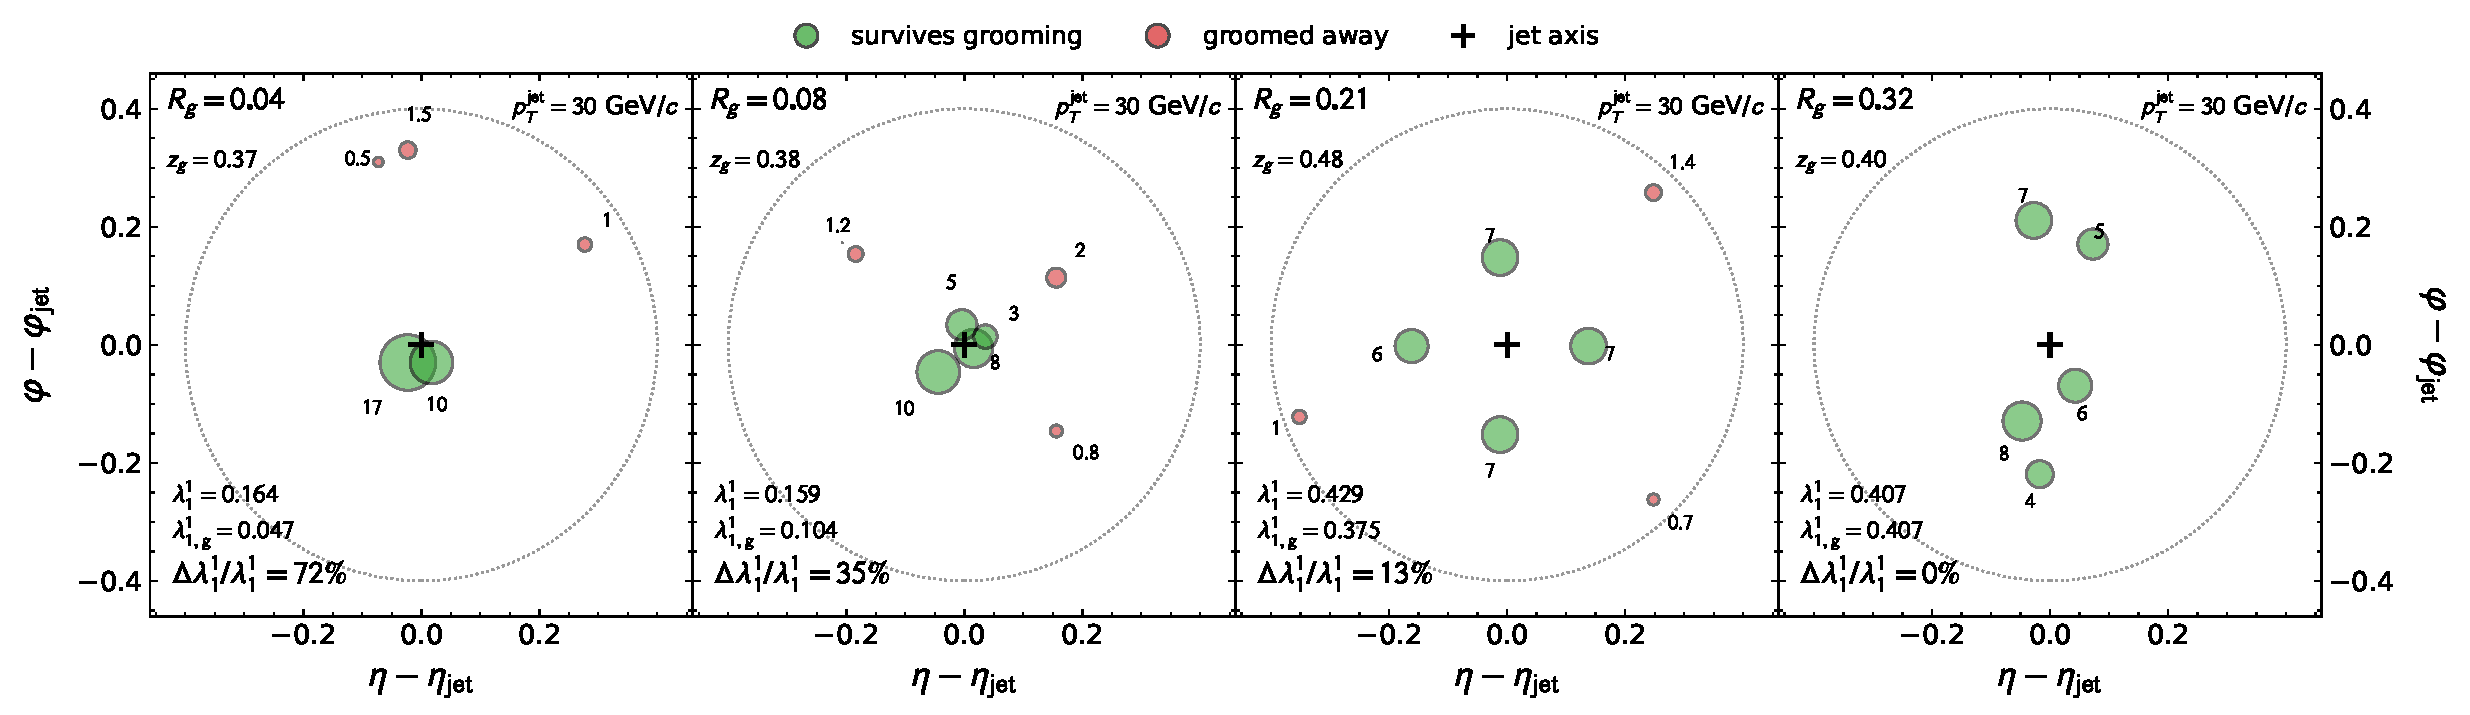
\includegraphics[width=\linewidth]{figures/fig_grooming_cartoon_4panel.pdf}
	\caption{ Ways of arranging constituents (each represented as a circle whose radius represent \(\frac{p_\mathrm{T, const}}{p_\mathrm{T, jet}}\)) in the \etaphi space within a jet with \(p_\mathrm{T, jet} = 30~\text{GeV}/c\) such that \(R_\mathrm{g}\) of the jet increases going from left to right. Green (Red) colored constituents survive (are removed by) the SoftDrop grooming ( \(z_\mathrm{cut} = 0.2,~\beta = 0\)).}
\end{figure}

\section{Analysis details}
\subsection{Dataset and Selections}
The analysis uses data from \pp collisions at \sPP{200}{GeV}~collected in 2012 using the STAR detector system. Charged-particle tracks and neutral energy depositions (towers) are measured using STAR's Time Projection Chamber (TPC) \cite{Anderson_2003} and Barrel Electromagnetic Calorimeter (BEMC) \cite{BEDDO2003725} detectors respectively. 

To enhance jet signal, only High-Tower (HT) triggered events, with at least one tower with $\EtTower \geq 4$ GeV are considered. Events containing a track with \ptGeq{track}{30} are rejected to avoid contamination from cosmic rays. Tracks(Towers) with \ptGeq{track}{0.2} (\(E_\mathrm{T, tower} \geq 0.2\) GeV) are considered for jet clustering. Clustered jets completely falling within acceptance ($|\eta_{\rm jet}| \leq 0.6$), with \ptGeq{jet}{10} and a plurality of charged tracks (\(N_\mathrm{ch., jet} \geq 2\)) are used for further study.  
%Jets with area, $A_{\rm jet} < 0.3$ are rejected to further reduce the fake jet contribution. 

 The tracks and towers are clustered into jets using the anti-\(k_{\rm T}\) algorithm with a jet resolution parameter $R = 0.4$, implemented using the FastJet library~\cite{Cacciari_2012}.  After obtaining the jets, the softer constituents are groomed using Recursive SoftDrop with \(\beta = 0\) and \(z_\mathrm{cut} = 0.2\). The groomed-jet's constituents lose non-kinematic information like charge, which is regained by matching them to the original jet's constituents. 
 
 \subsection{Detector effects and Unfolding}
 The embedding simulation starts from PYTHIA6 (STAR Tune)  at the particle level. The particles are then reconstructed as detector hits using the STAR detector system implemented in GEANT3 and embedded into zero-bias events from 200 GeV \pp collisions (2012). The jets from particle and detector levels are matched using a \(p_\mathrm{T, jet}\) ordered nearness criteria.  The matched jets can be used to show detector responses like shown in Fig. \ref{fig:PtResonse} 
 
 \begin{figure}[h]
 	\centering
 	\label{fig:PtResonse}
 	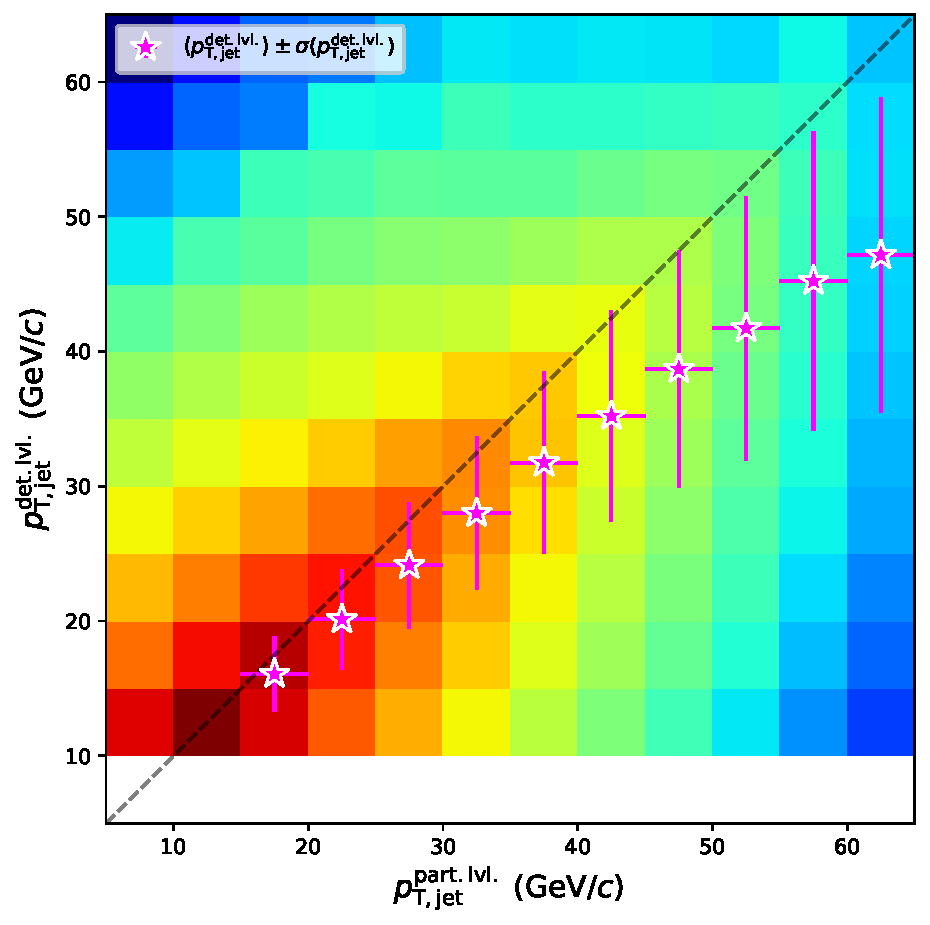
\includegraphics[width=0.5\linewidth]{figures/jet_pt_response.pdf}
 	\caption{Two-dimensional histogram showing detector response for \(p_\mathrm{T, jet}\), showing probability of a \ptGenJet particle level jet being reconstructed as \ptRecoJet. Purple stars shows expected \ptRecoJet given a particular bin of the \ptGenJet.}
 \end{figure}
 \(p_\mathrm{T, jet}\)-resolution shown in Fig. \ref{fig:PtResolution}.  
 \begin{figure}[h]
 	\centering
 	\label{fig:PtResolution}
 	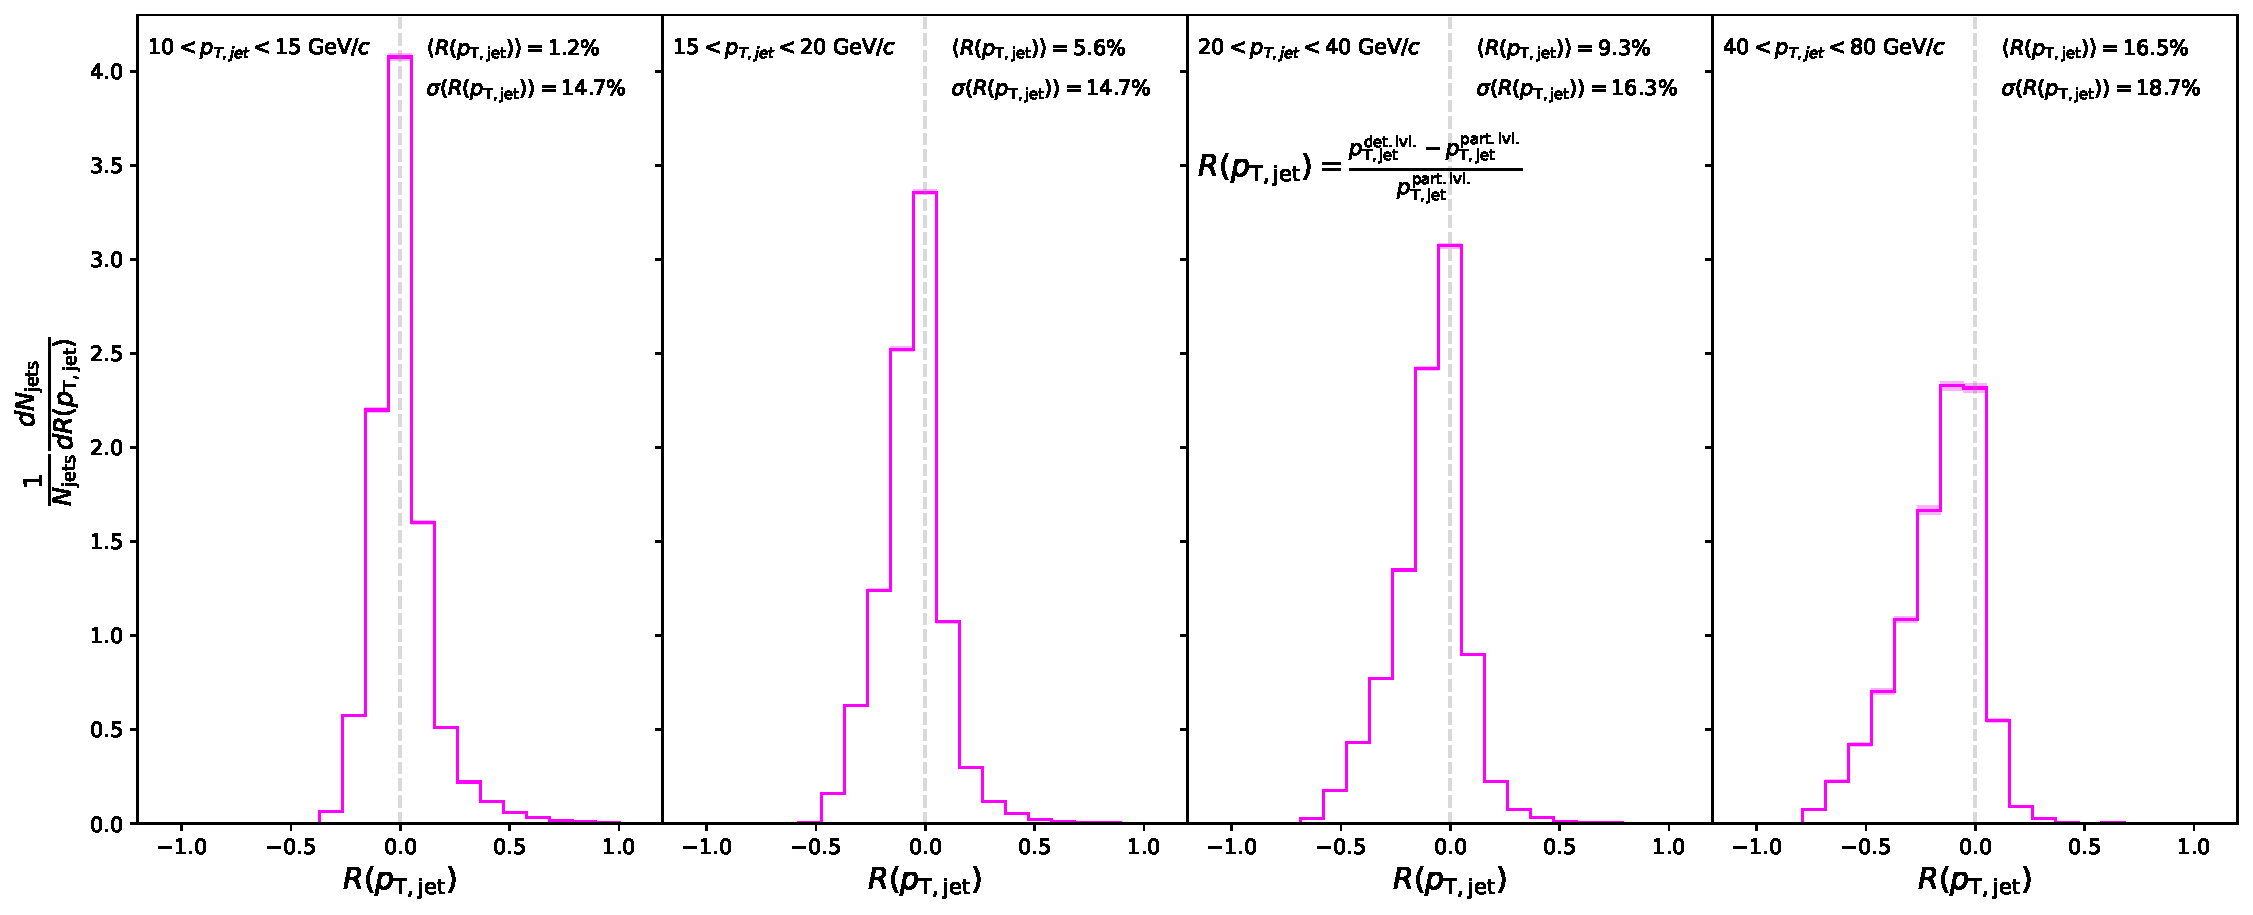
\includegraphics[width=\linewidth]{figures/jet_pt_res.pdf}
 	\caption{\(p_\mathrm{T, jet}\)-resolution in different \(p_\mathrm{T, jet}\) bins.}
 \end{figure}
 
 Unfolding is done using the Multifold method. Every jet is represented as a vector of 23 features. The four classifiers of Multifold are parametrized as DNNs with 3 hidden layers with 256 nodes each. The model weights are trained using the AdamW optimizer with a learning rate of \(10^{-3}\) and weight decay of \(10^{-2}\). Convergence is achieved in two unfolding iterations. Statistical uncertainties are calculated using bootstrap ensemble with 50 model replicas each sub-sampling  500k each of the data-like and sim-like jets, so each model replica sees 1M jets every epoch. All the  required unfolded distributions and profiles are calculated by using the per-jet unfolding weights. 
 
 Closure test of the unfolding shown in  Fig. \ref{fig:ClosureAngularities} is done by doing the same unfolding procedure replacing measured data with pseudo-data for which the particle level is known (pseudo-truth). The pseudo-unfolded distributions are then compared to the pseudo-truth via ratios
 \begin{figure}[h]
 	\centering
 	\label{fig:ClosureAngularities}
 	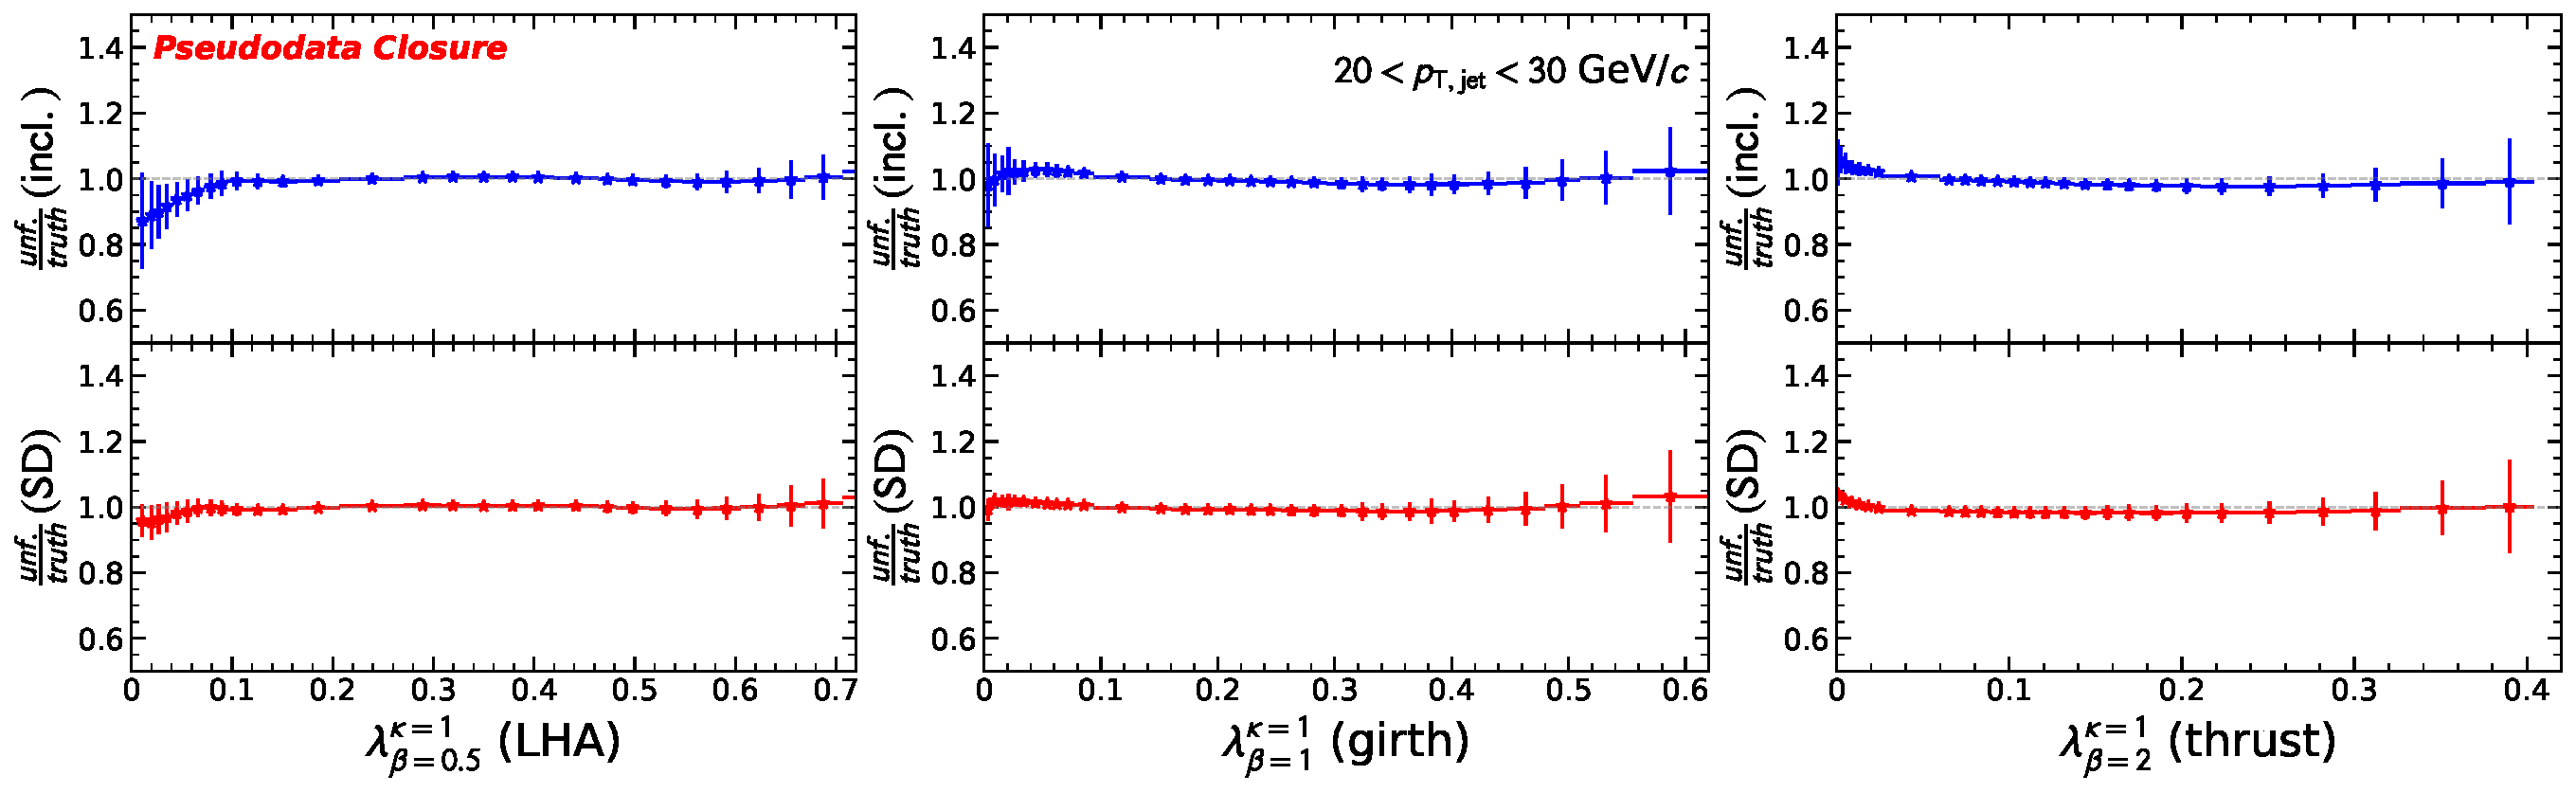
\includegraphics[width=\linewidth]{figures/fig_dist_grid_closure_like.pdf}
 	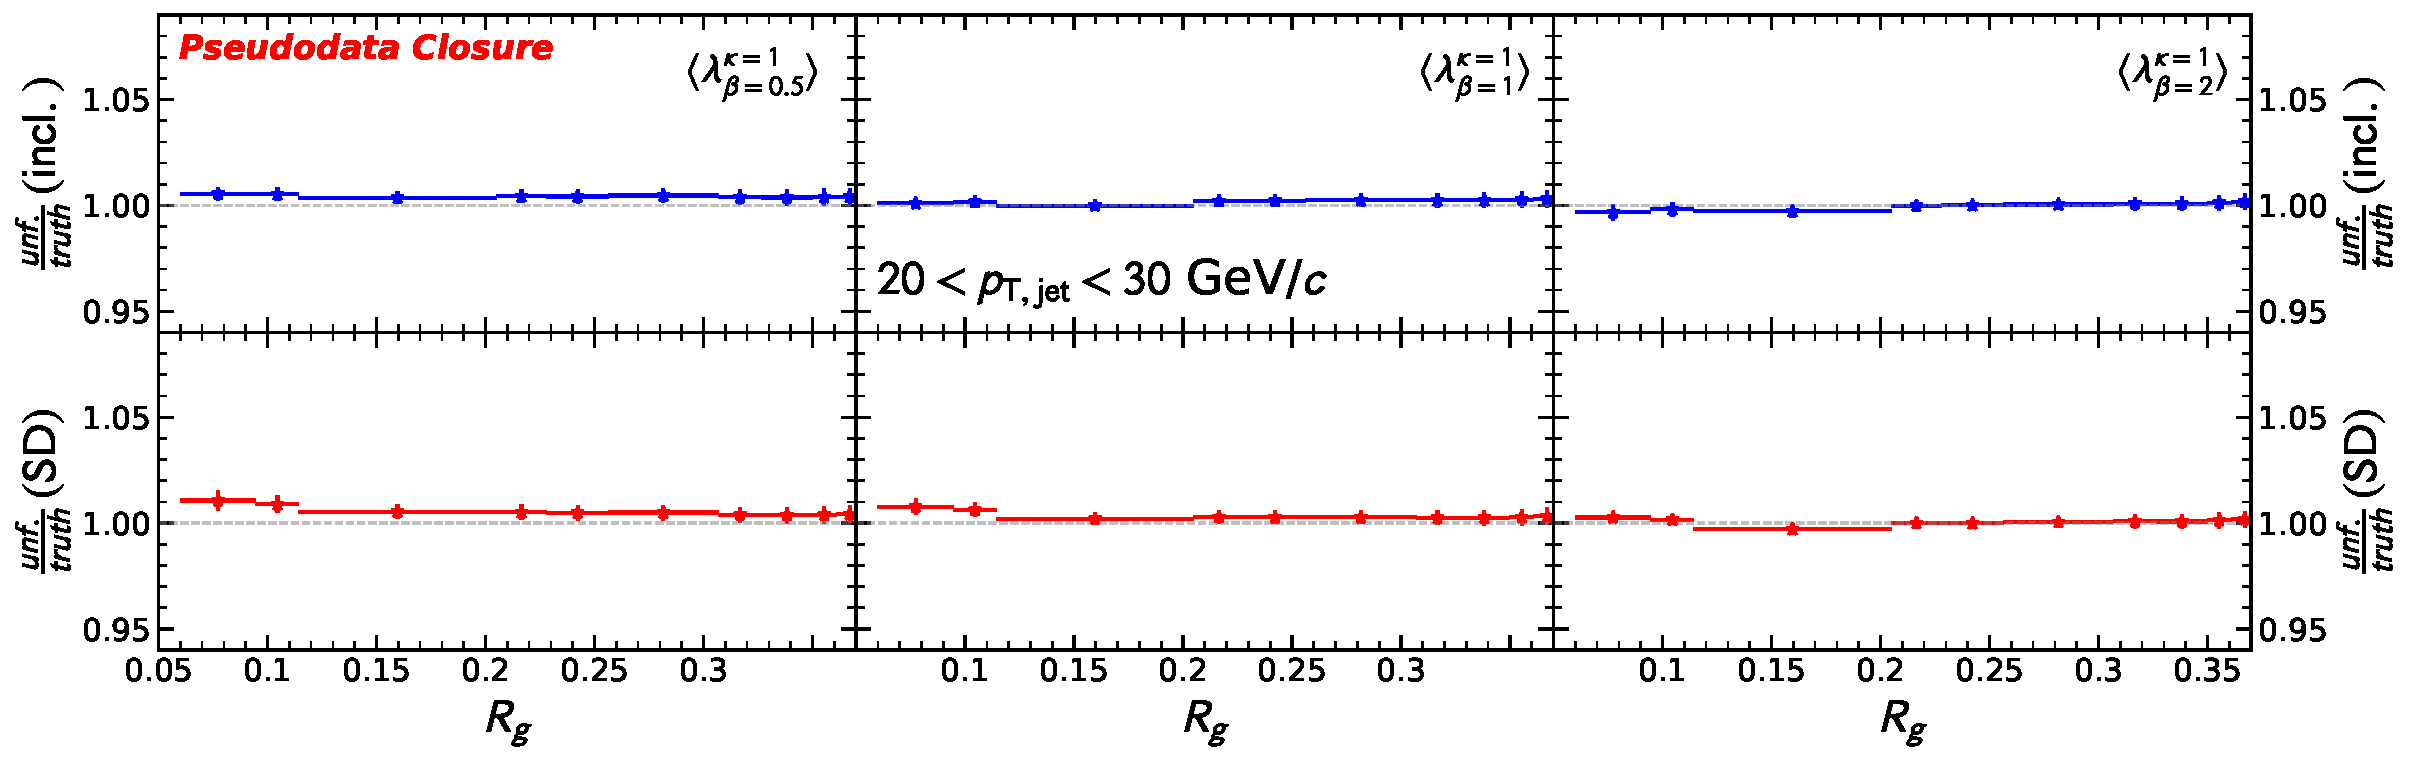
\includegraphics[width=\linewidth]{figures/fig_dr_grid_closure_like.pdf}
 	\caption{Closures for \(\lambda^{\kappa=1}_{\beta\in\{0.5, 1, 2\}}\) distributions (top) and \(R_\mathrm{g}\) profile (bottom) shown for jets with \ptRange{jet}{20}{30}.}
 \end{figure}
 
 \subsection{Systematic Uncertainties}
 
 
\section{Results}
\begin{figure}[h]
	\centering
		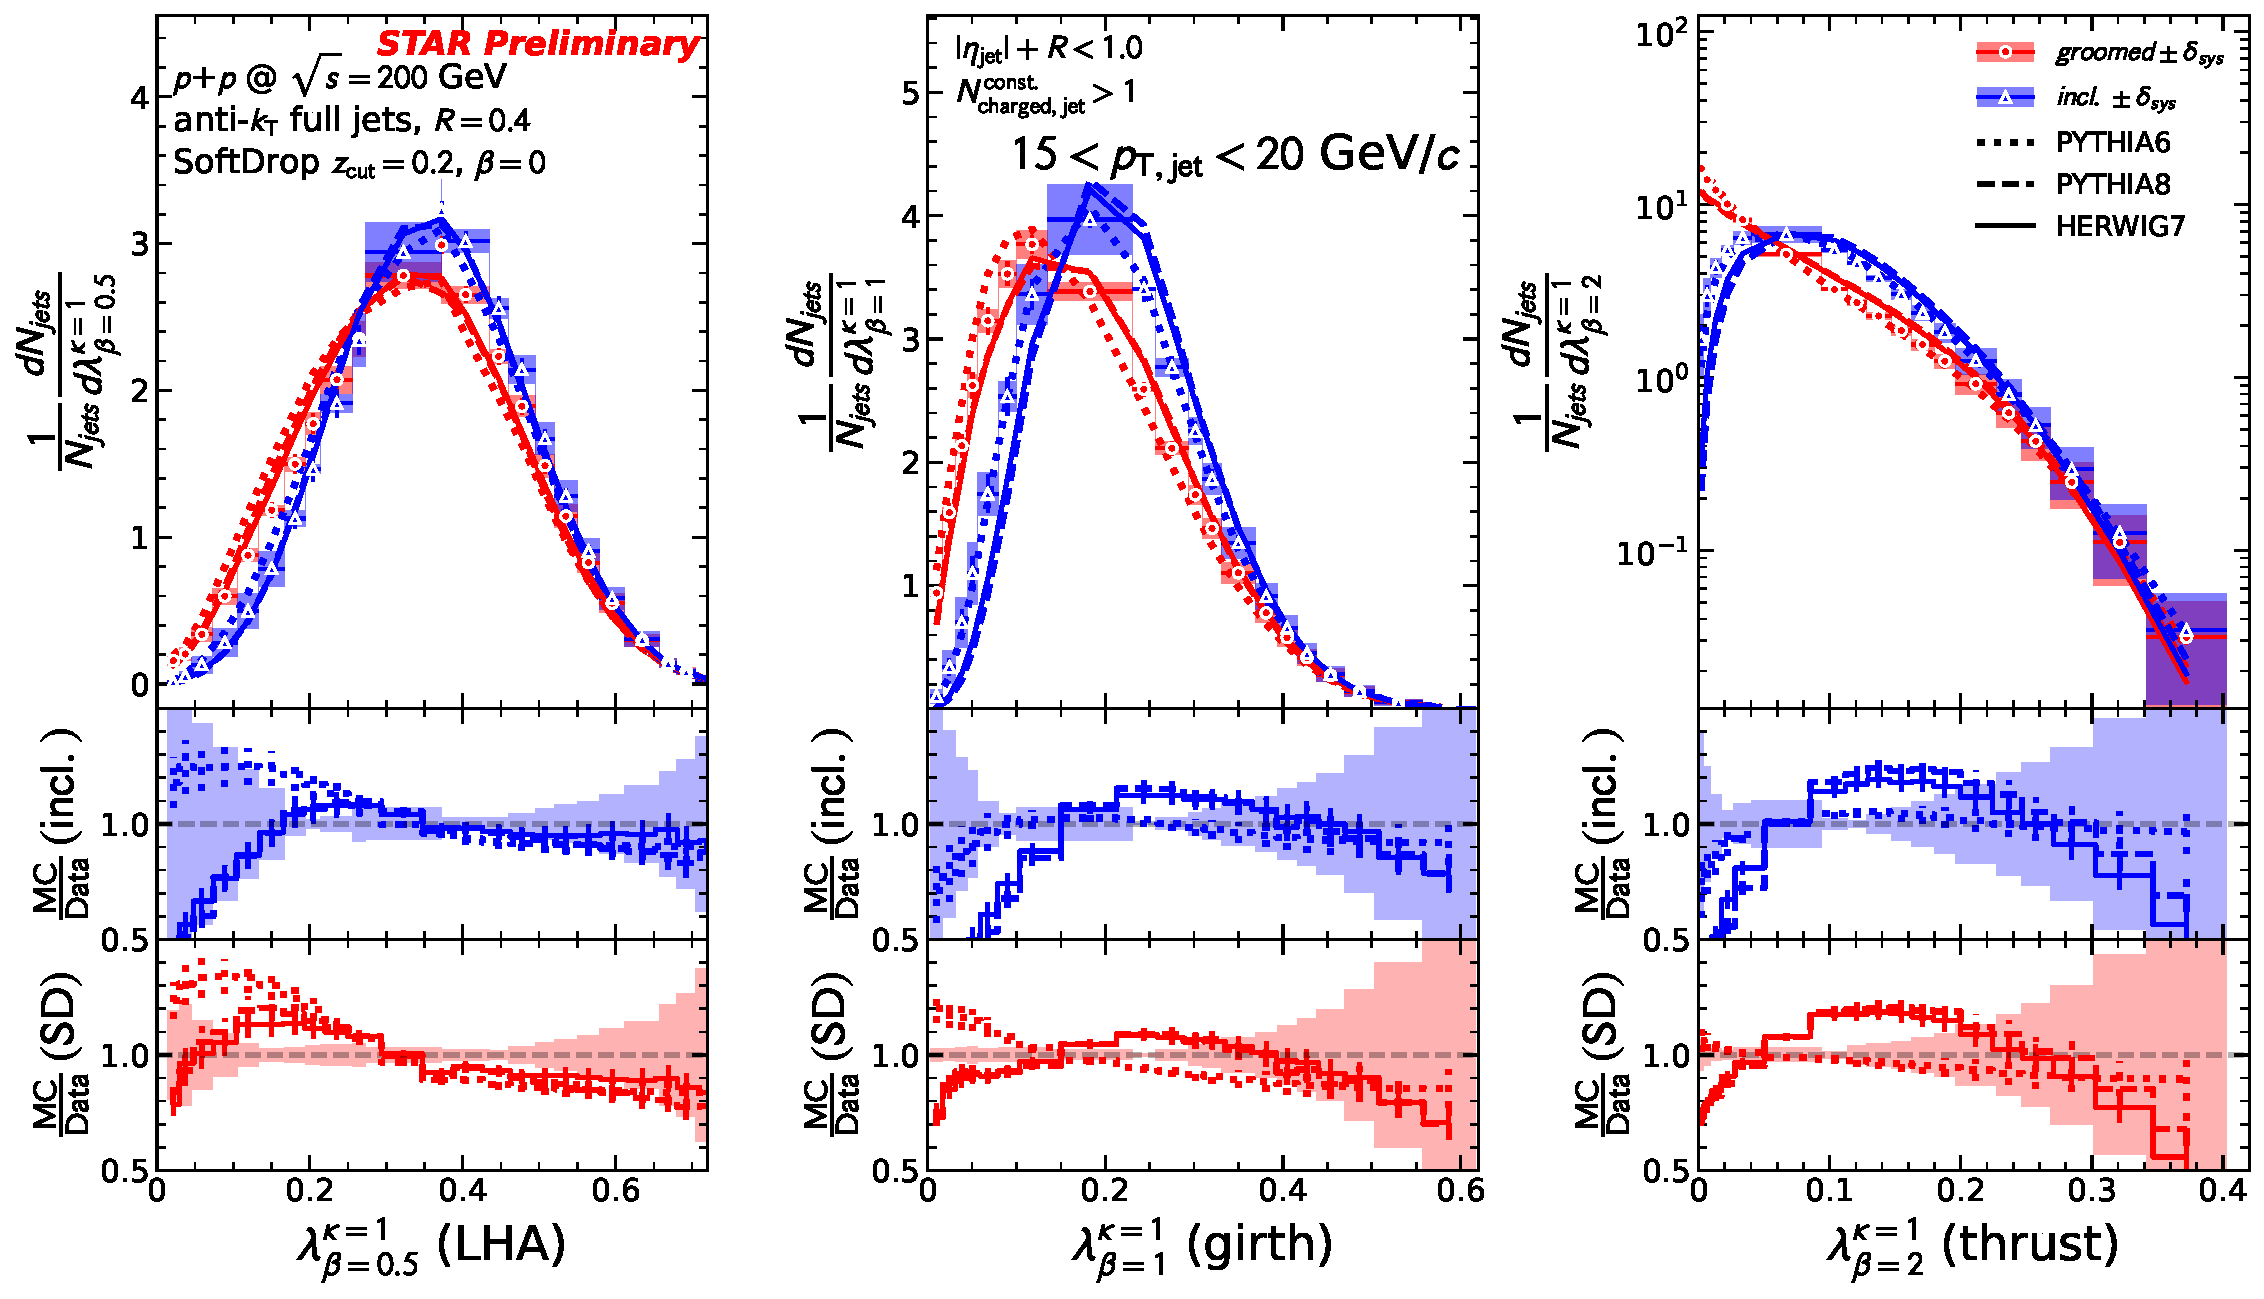
\includegraphics[width=0.8\linewidth]{figures/fig_grid_jpt1.pdf}
	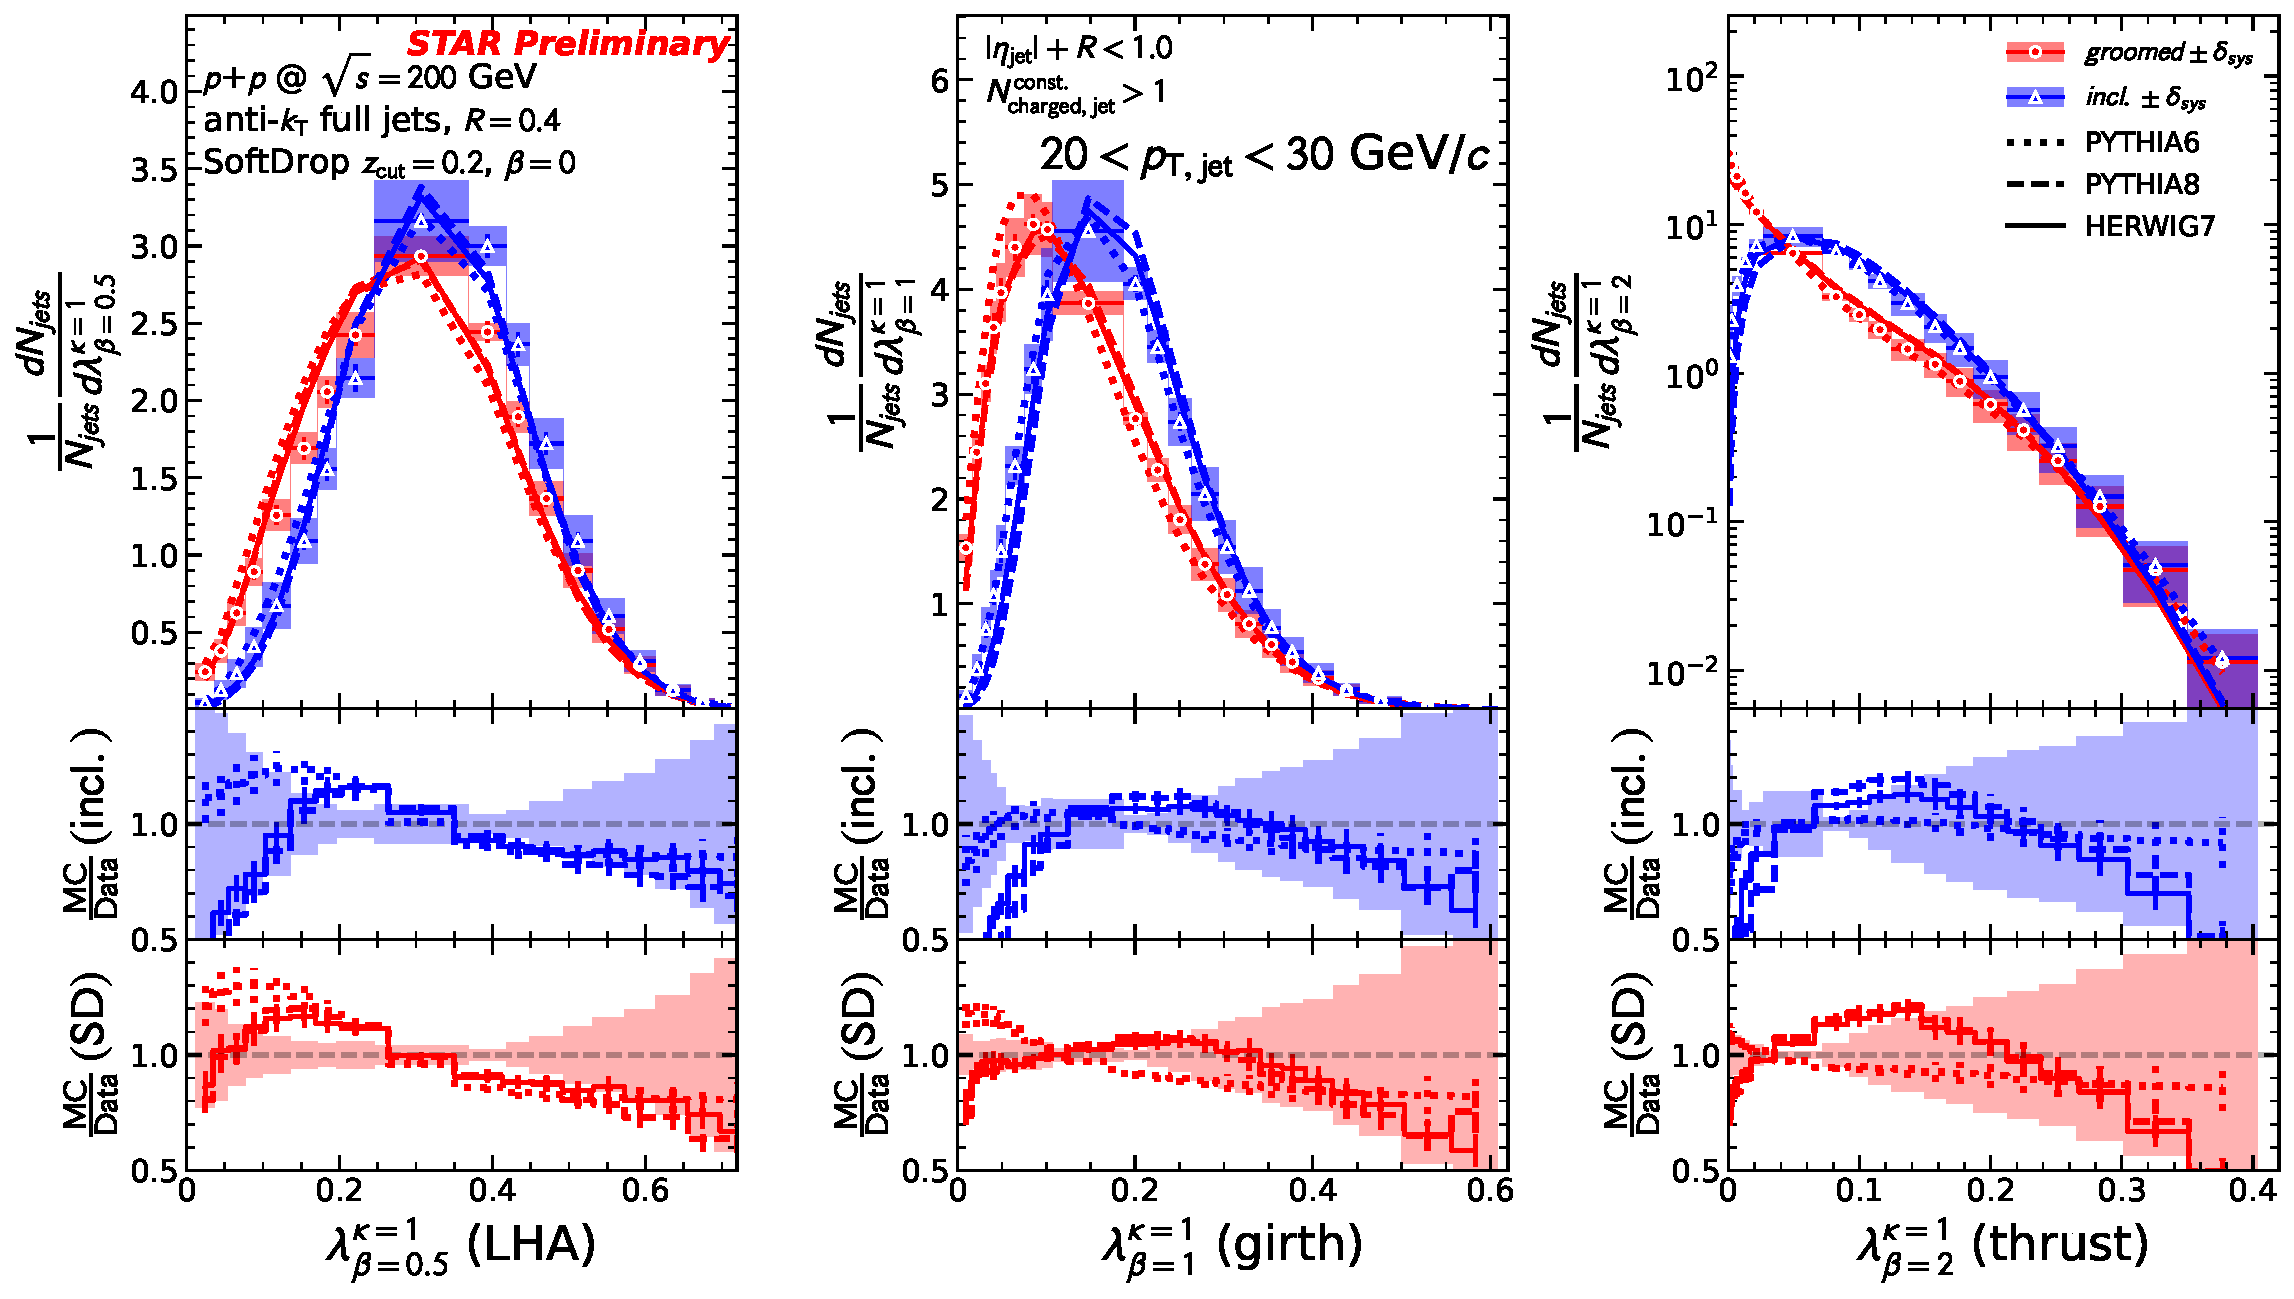
\includegraphics[width=0.8\linewidth]{figures/fig_grid_jpt2.pdf}
		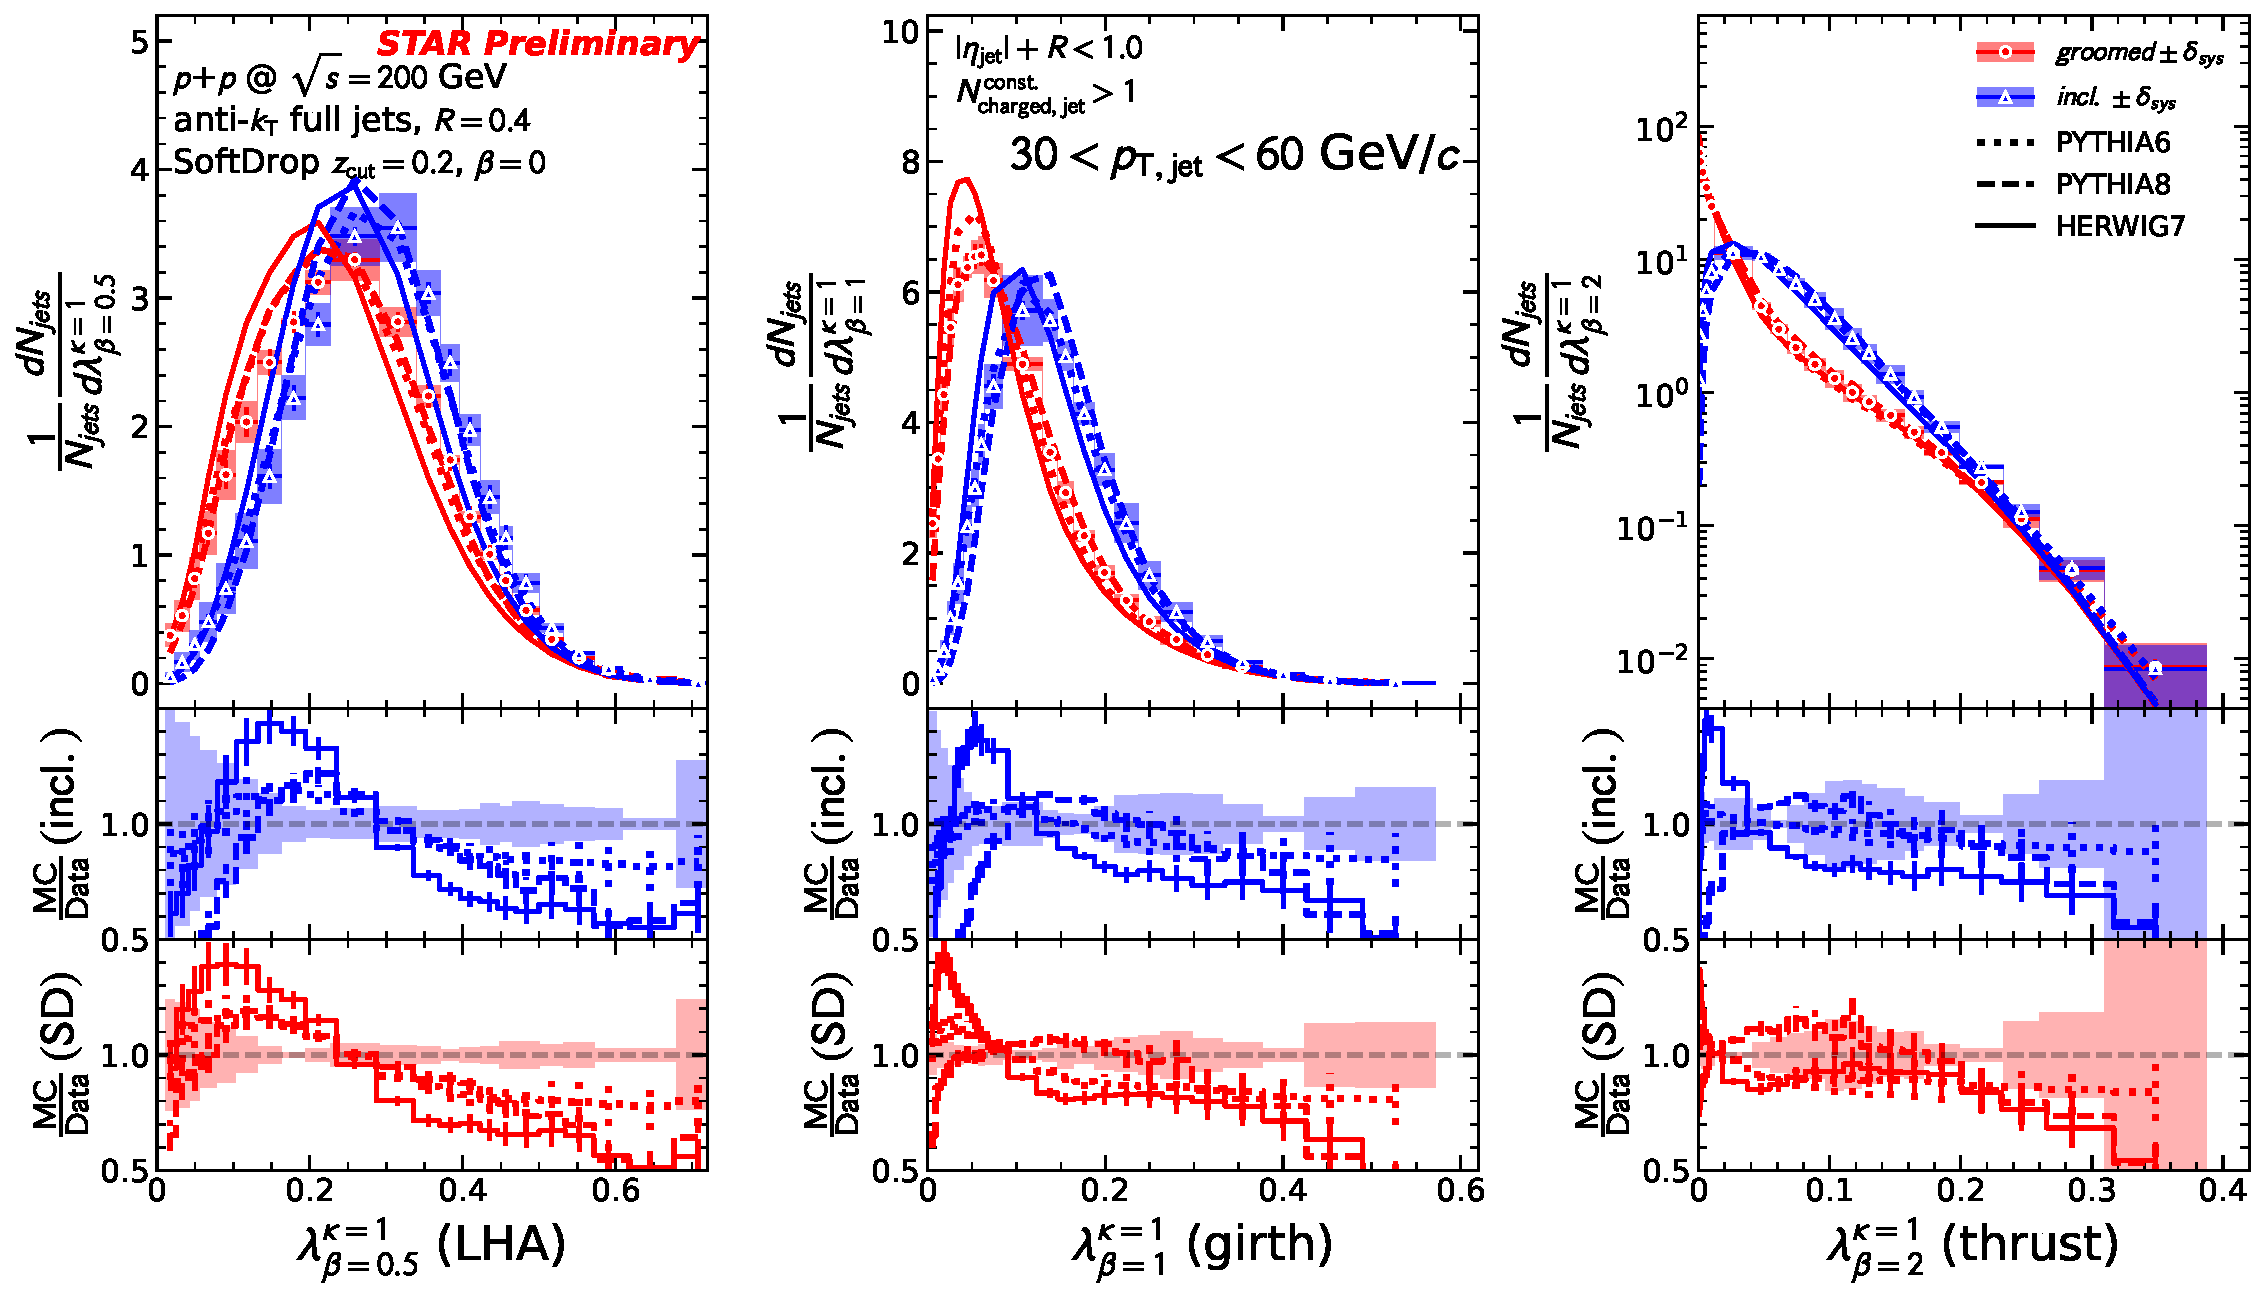
\includegraphics[width=0.8\linewidth]{figures/fig_grid_jpt3.pdf}
\end{figure}
\begin{figure}[h]
	\centering
		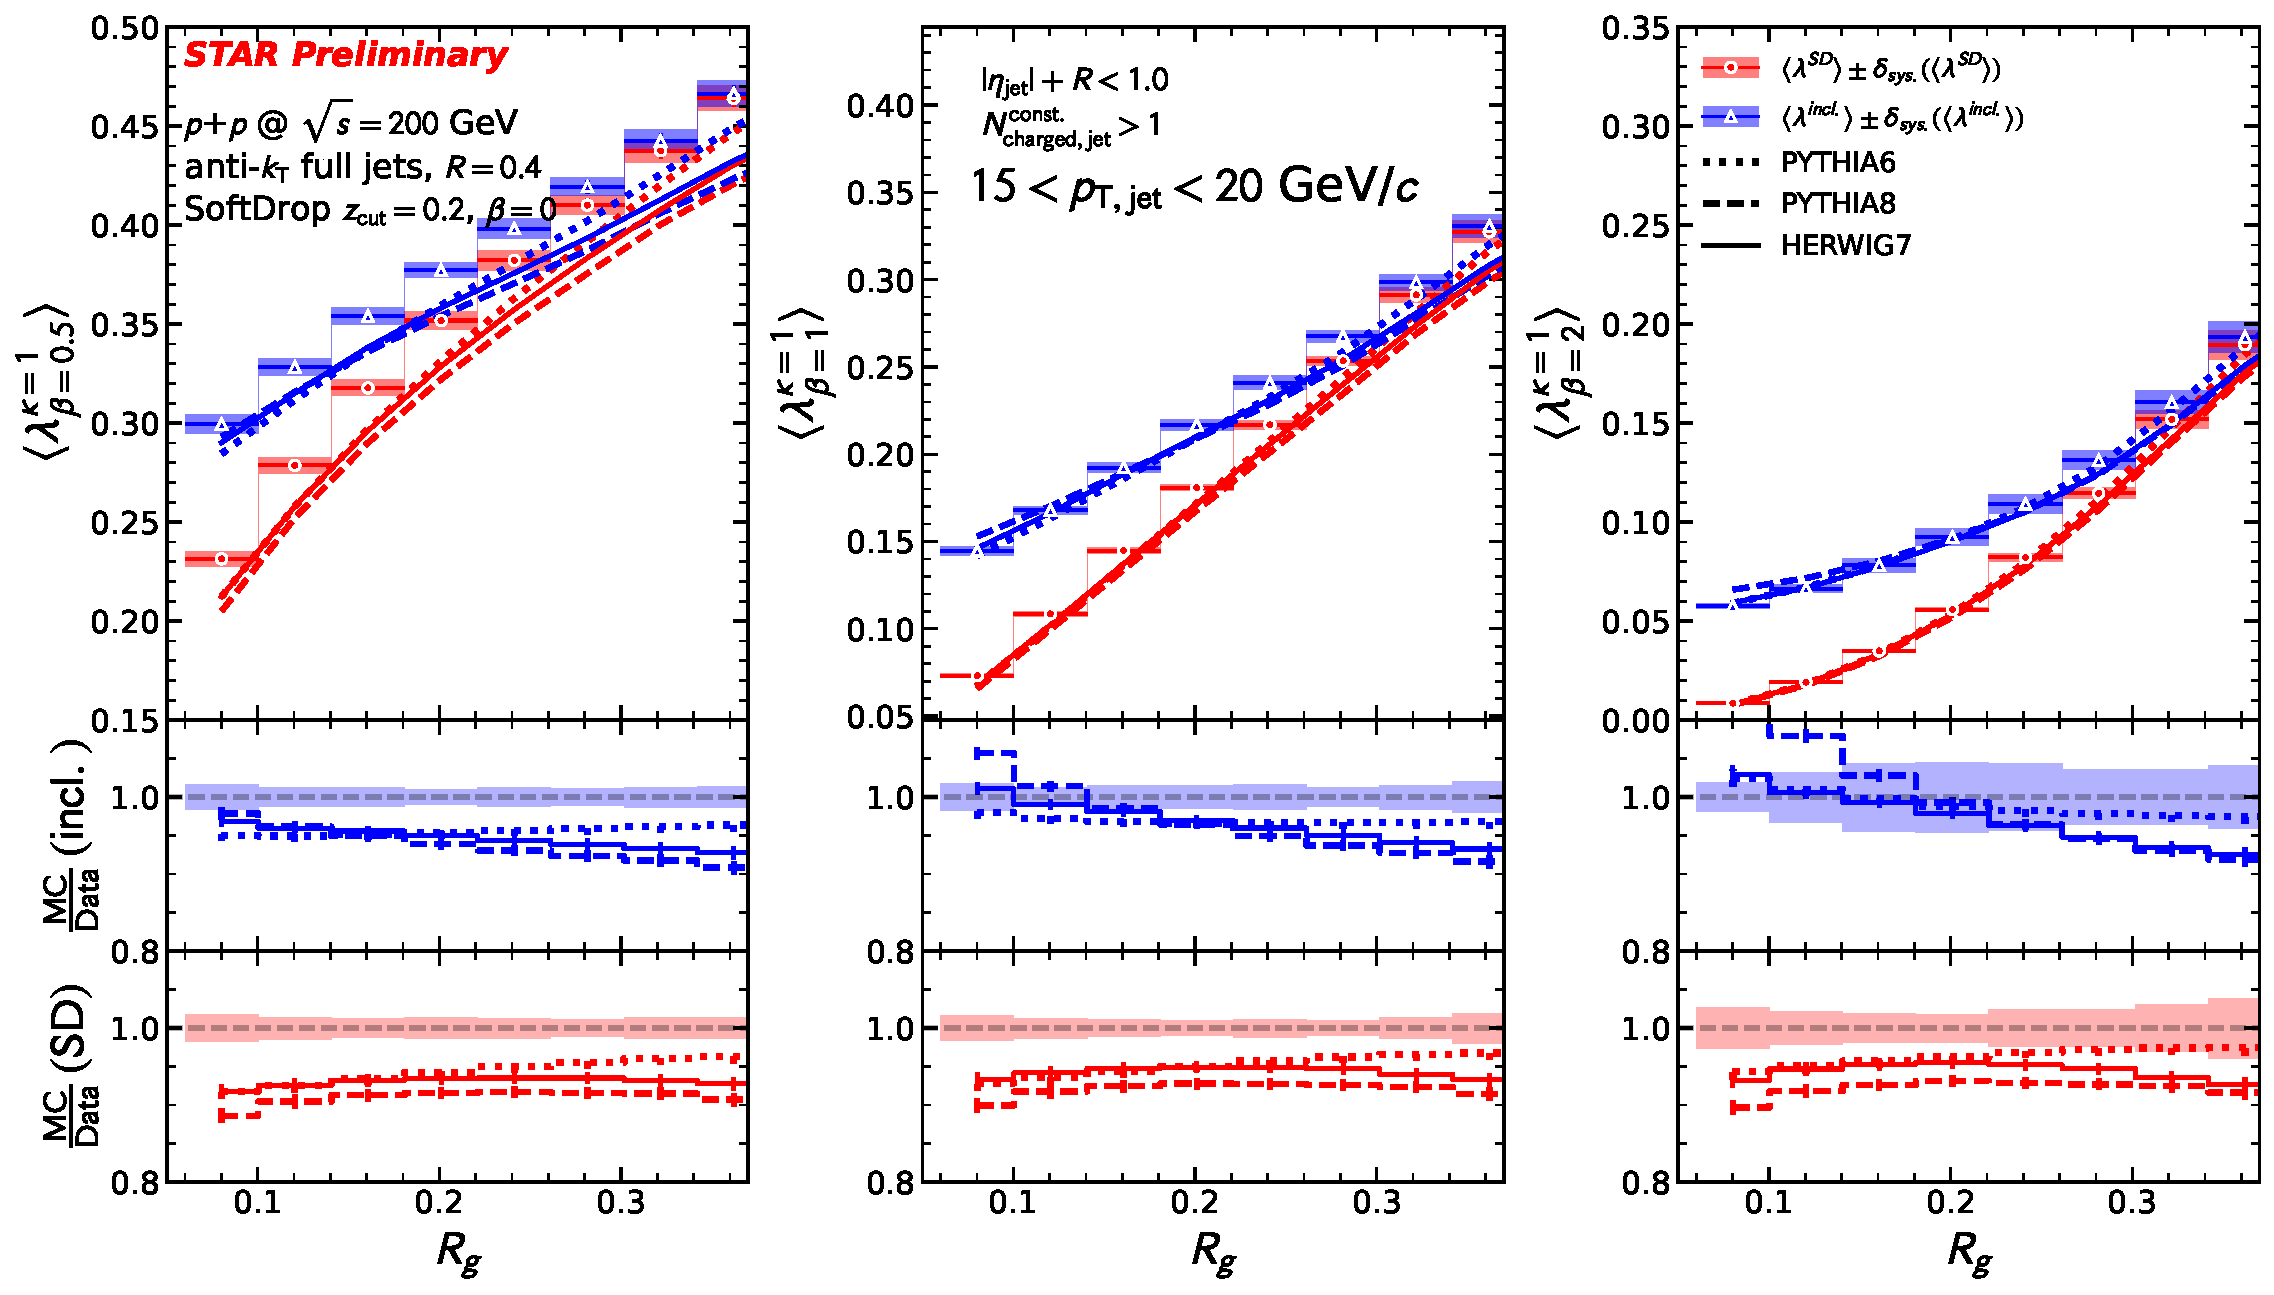
\includegraphics[width=0.8\linewidth]{figures/fig_prof_grid_jpt1.pdf}
			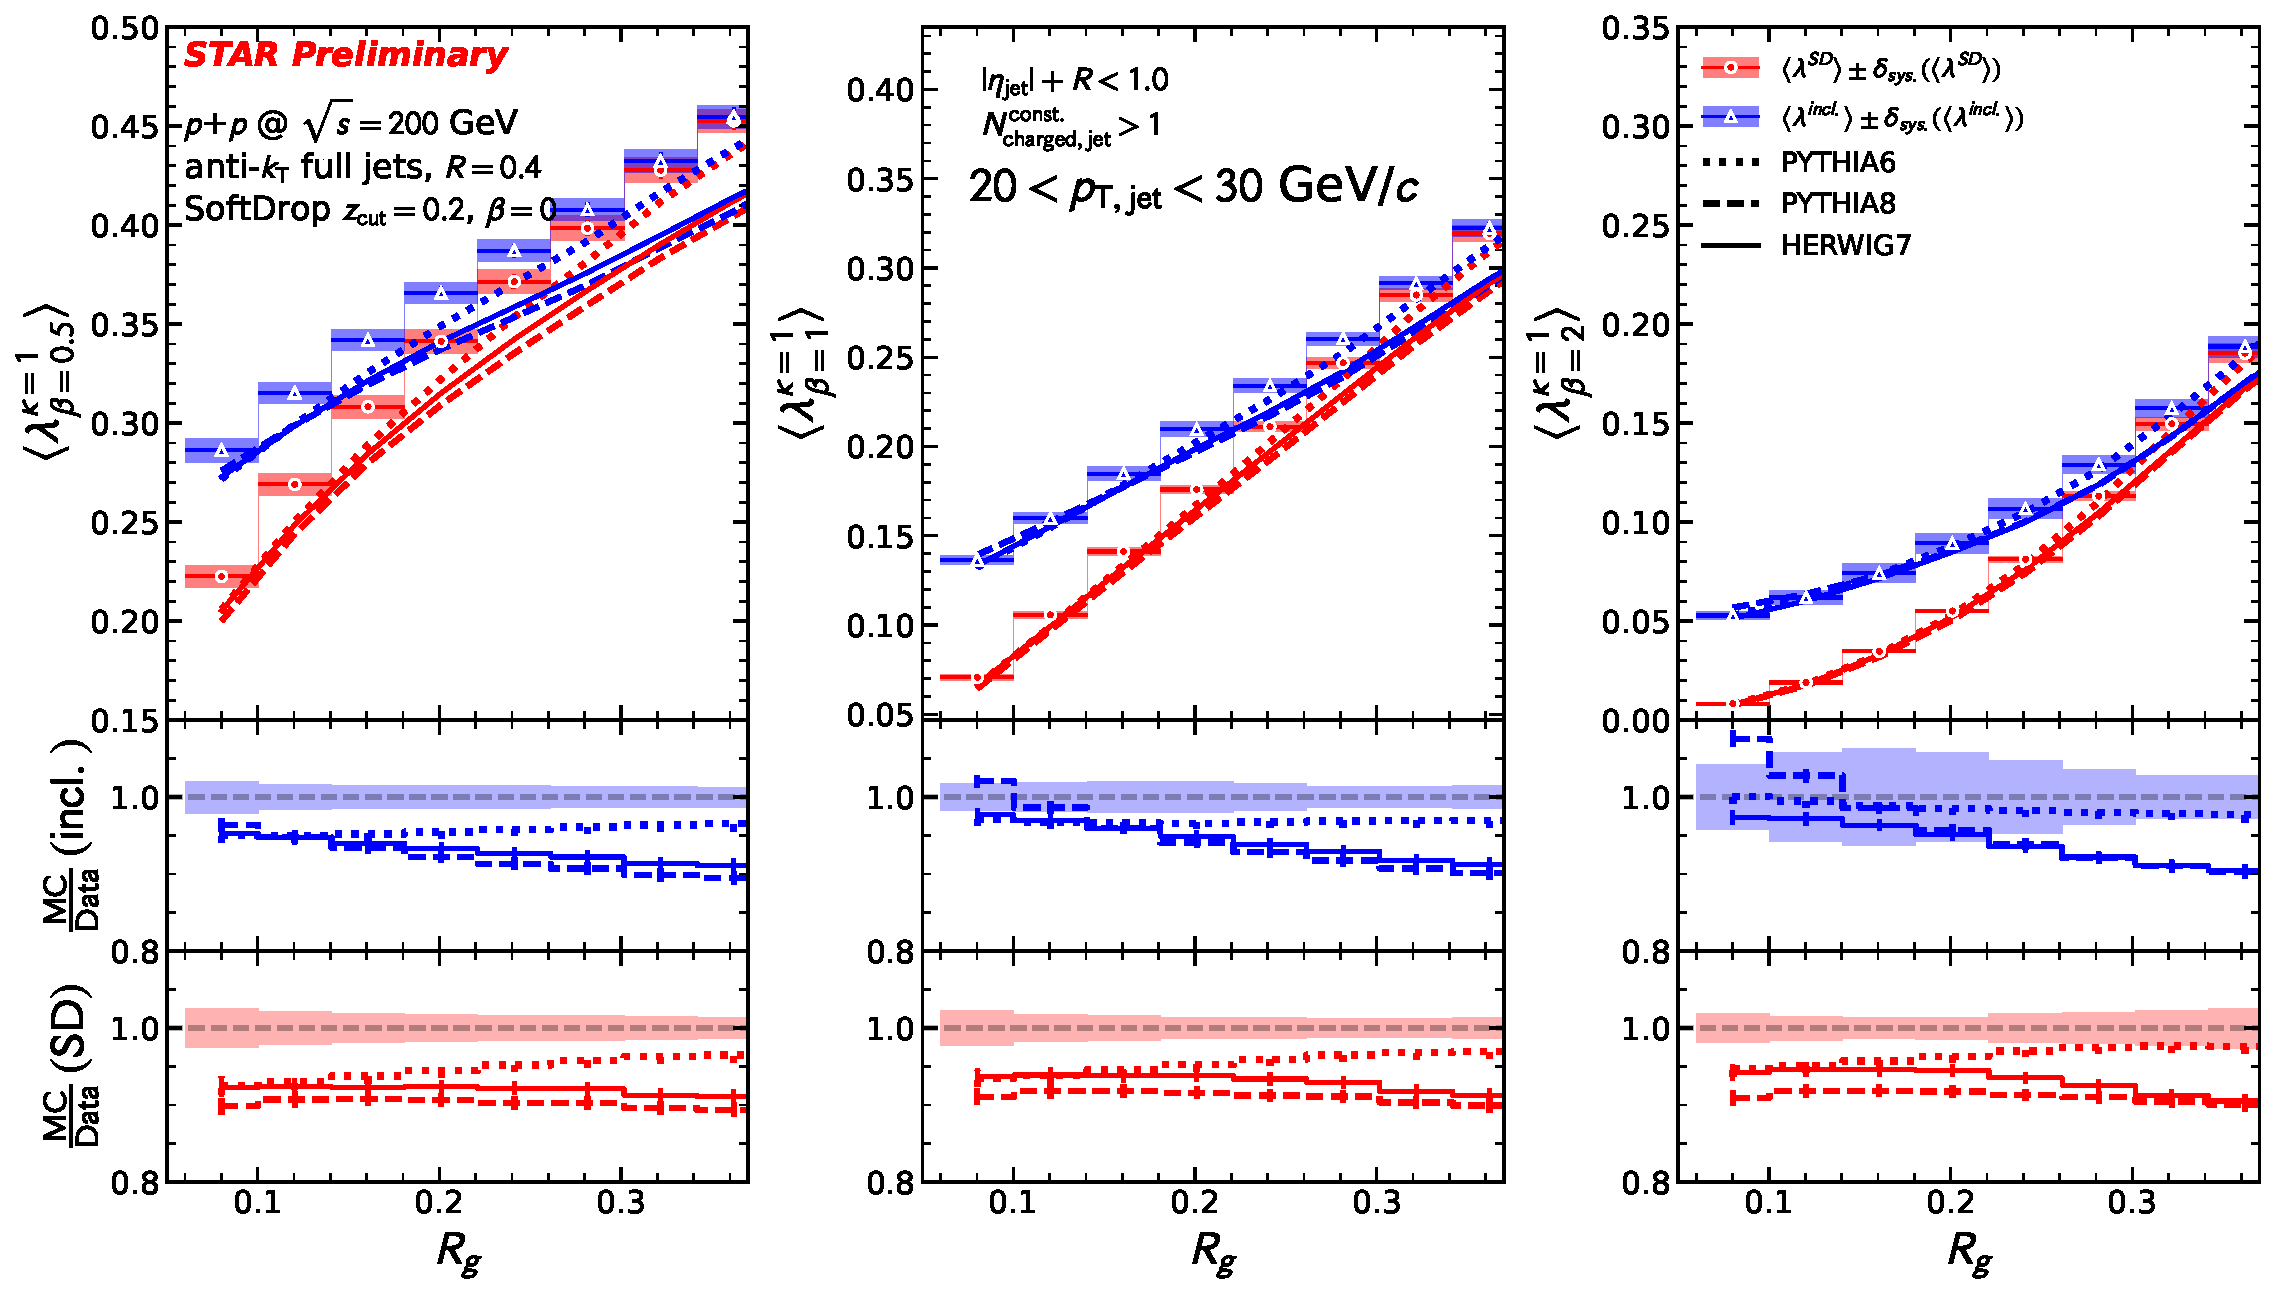
\includegraphics[width=0.8\linewidth]{figures/fig_prof_grid_jpt2.pdf}
	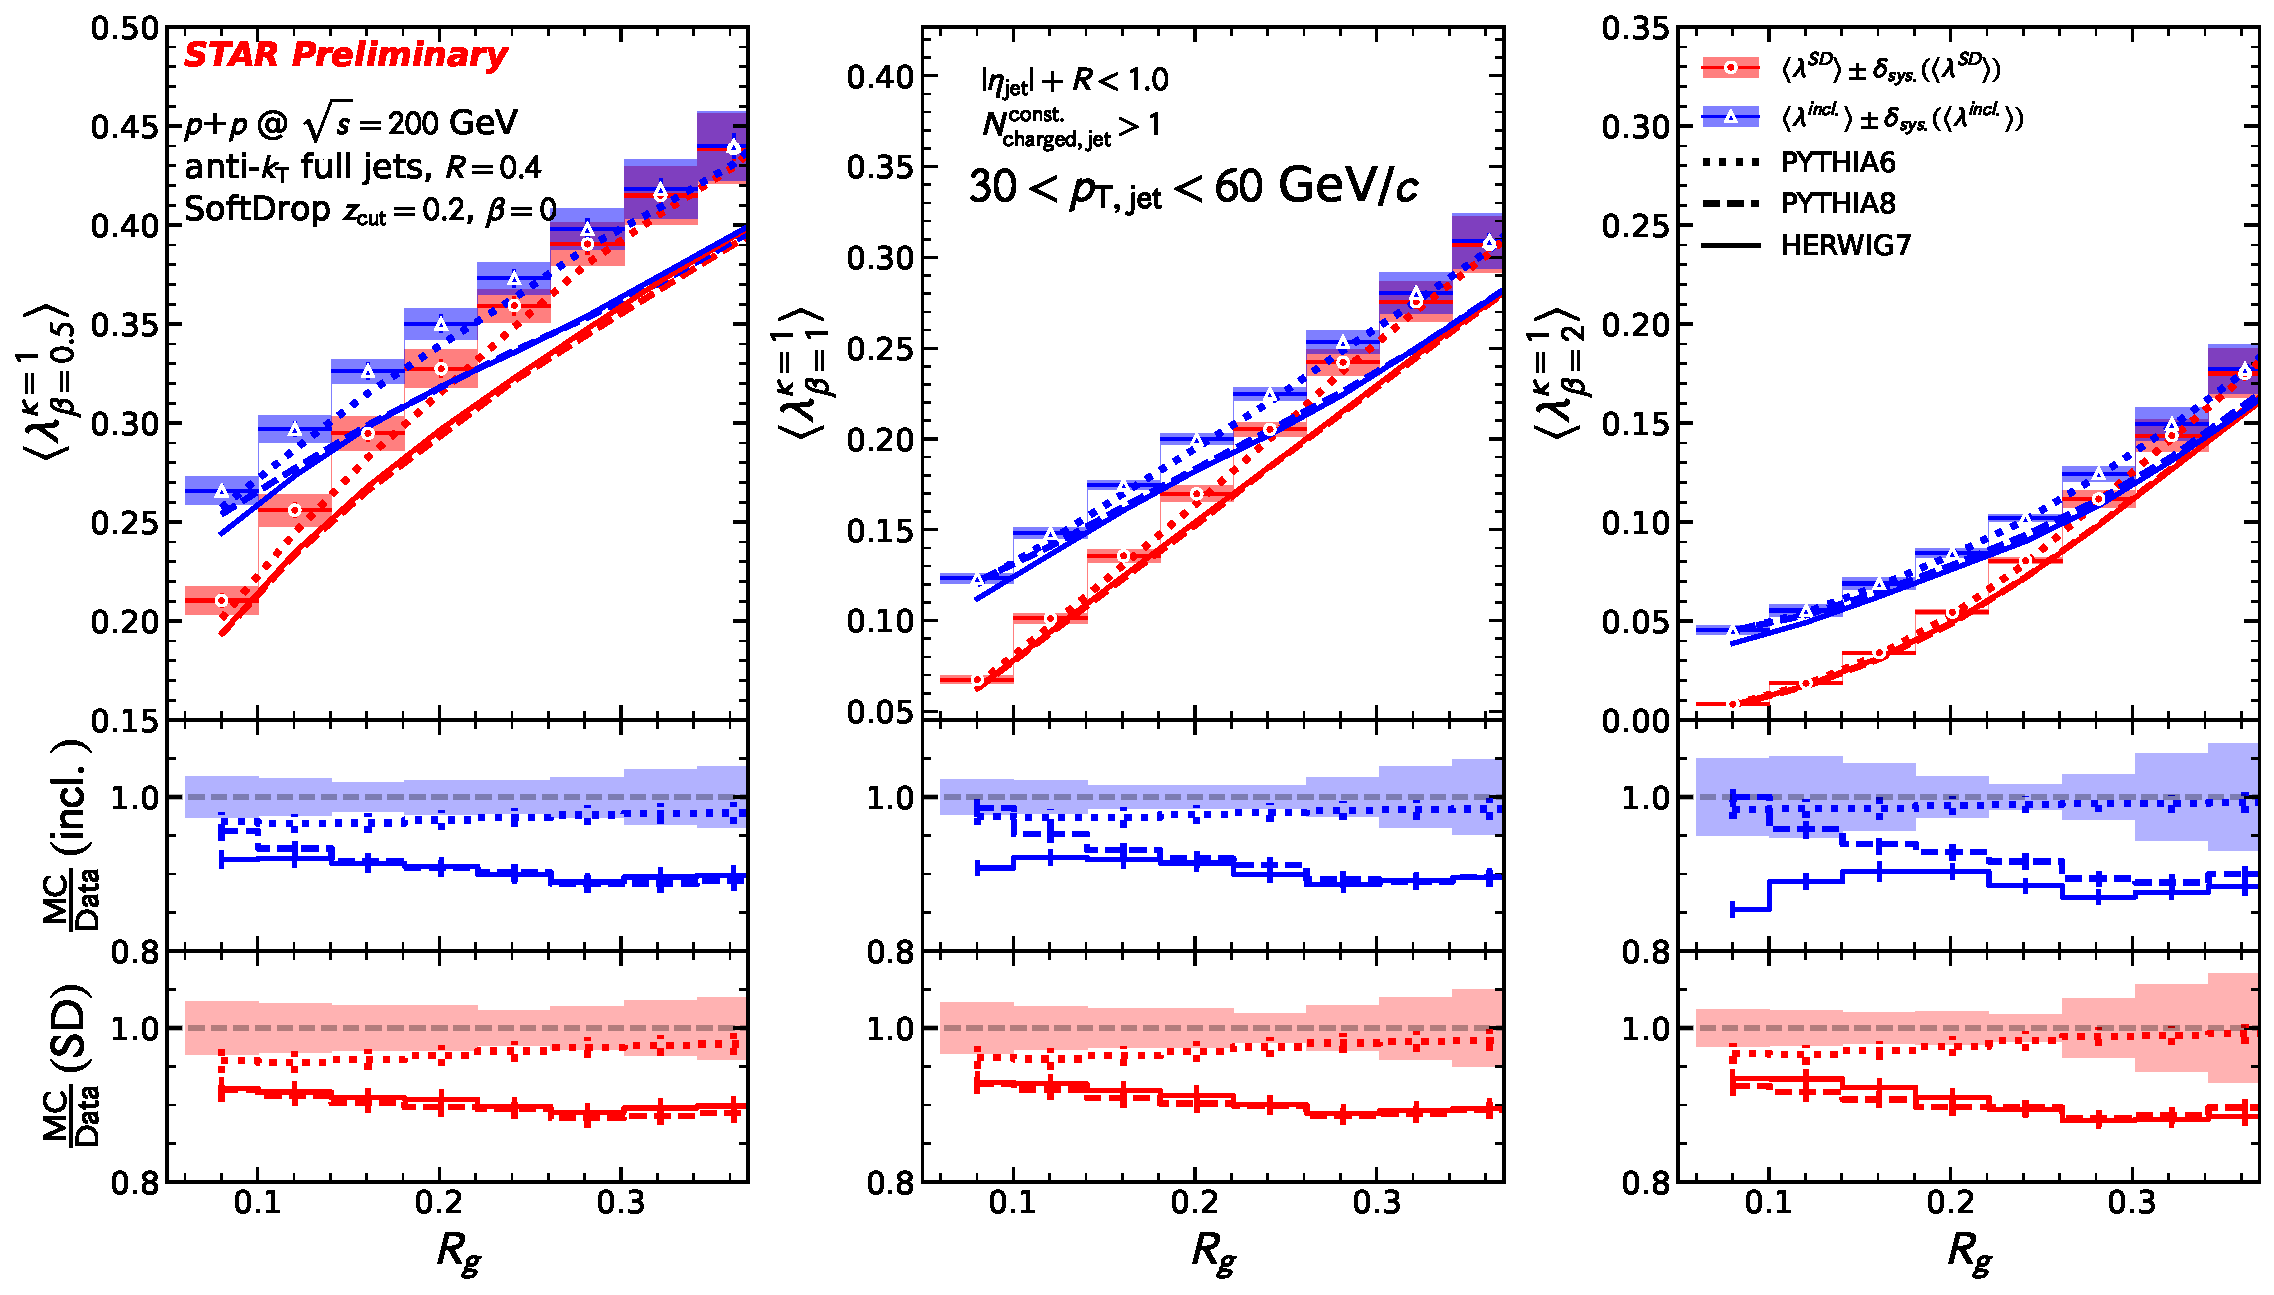
\includegraphics[width=0.8\linewidth]{figures/fig_prof_grid_jpt3.pdf}
\end{figure}

\section{Conclusion and Outlook}


